\documentclass[12pt,a4paper]{article}
\usepackage[letterpaper]{geometry}
\geometry{top=1.0in, bottom=1.0in, left=1.0in, right=1.0in}
\usepackage{setspace} \doublespacing
\usepackage{titlesec}
\usepackage{natbib}
\bibliographystyle{abbrv}
\usepackage{url}

\usepackage{subcaption}
\usepackage{graphicx}

\begin{document}
\paragraph{Motivation and target audience}
    According to the UK-office of National Statistics \citep{ONSstats}, there are nearly 12 million people aged 65 and above in the UK, and falls are the largest cause of non-fatal emergency hospital admissions for older people \citep{NHSInjuries}.
    About half of people aged 80+ fall at least once a year, and can cause not only injury, but also a loss of confidence and independence.
    In 2017/18 there were approximately 220,000 emergency hospital admissions related to falls among patients aged 65+, with about 66\% being aged 80+ \citep{GovUKFalls}.

    While we may not be able to prevent falls, we can improve the chances of an elderly individual to find the immediate help they need following an accident.

\paragraph{Purpose}
    To provide a way for an elderly couple and/or person who lives alone to communicate their need for assistance, especially after a fall.
    The app automatically notifies an emergency contact after a fall, provides one's location and, in case of a general emergency, an emergency call button. 

\paragraph{Alternatives}
    There are several applications in existence that provide certain aspects of our app -- Red Panic Button is a medical alert, Fall Detector; as well as stand-alone medical alert systems, such as ADT, Medical Alert and Bay Alarm Medical.

\paragraph{Technical development}
    In order to develop the application, we used the Matlab and Simulink software.

    We used the Accelerometer Block to determine whether the sum of the magnitudes of the accelerations in the x, y, and z axis is less than 4 in order to identify whether the sender device is falling.
    This value was determined experimentally. 
    The \textit{sender} phone continuously provides GPS coordinates using the Location Sensor block, and upon falling, the \textit{receiver} phone is notified by a beeping sound and a warning.
    The sender also has the option to press the Emergency Contact button to continuously produce a notification on the receiver’s phone. 

    Below are the diagrams of the app, as well as its interface.
    \begin{figure}[h]
        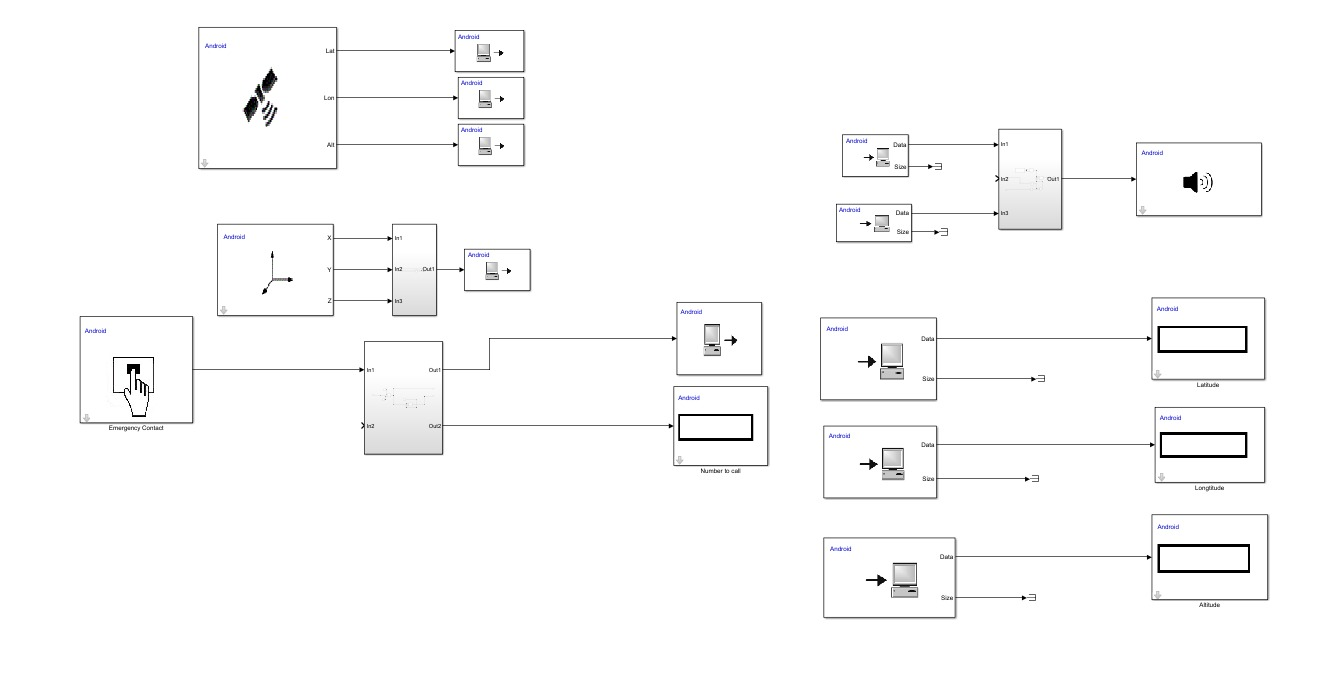
\includegraphics[width=\textwidth]{./files/Overview.jpeg}
        \caption{Application design. Accelerometer (\ref{fig:Acc}), emergency button (\ref{fig:EB}) and audio output (\ref{fig:AO}) are further explored below }
        \label{fig:Overview}
    \end{figure}
\begin{figure}[h]
    \centering
    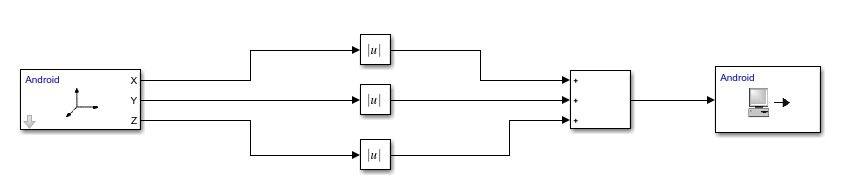
\includegraphics[width=\textwidth]{files/Accelerometer.jpeg}
    \caption{Accelerometer.}
    \label{fig:Acc}
\end{figure}
\begin{figure}[h]
    \centering
    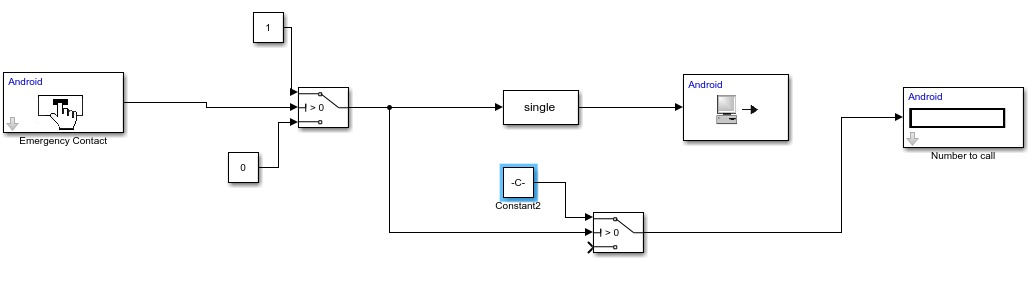
\includegraphics[width=\textwidth]{files/EmergencyButton.jpeg}
    \caption{Emergency button. Note Constant2 is the emergency phone number -- a work-around due to the inability to display a string.}
    \label{fig:EB}
\end{figure}
\begin{figure}[h]
    \centering
    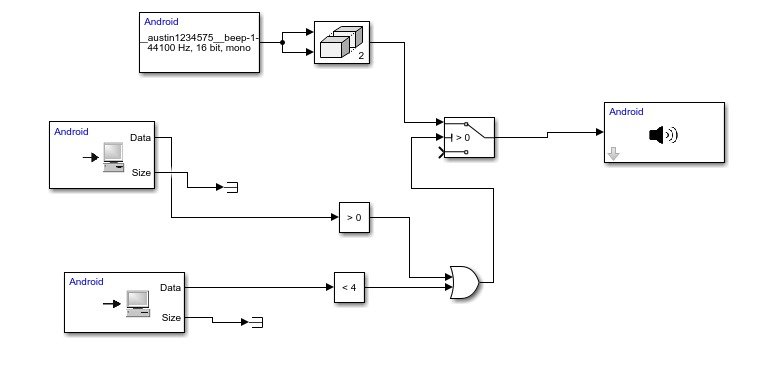
\includegraphics[width=\textwidth]{files/AudioOutput.jpeg}
    \caption{Audio output. The audio file's frame size (441) was changed according to the compiler's demand. Output frequency: 44100 Hz.}
    \label{fig:AO}
\end{figure}
\begin{figure}[h]
    \centering
    \begin{subfigure}[t]{0.4\textwidth}
        \centering
        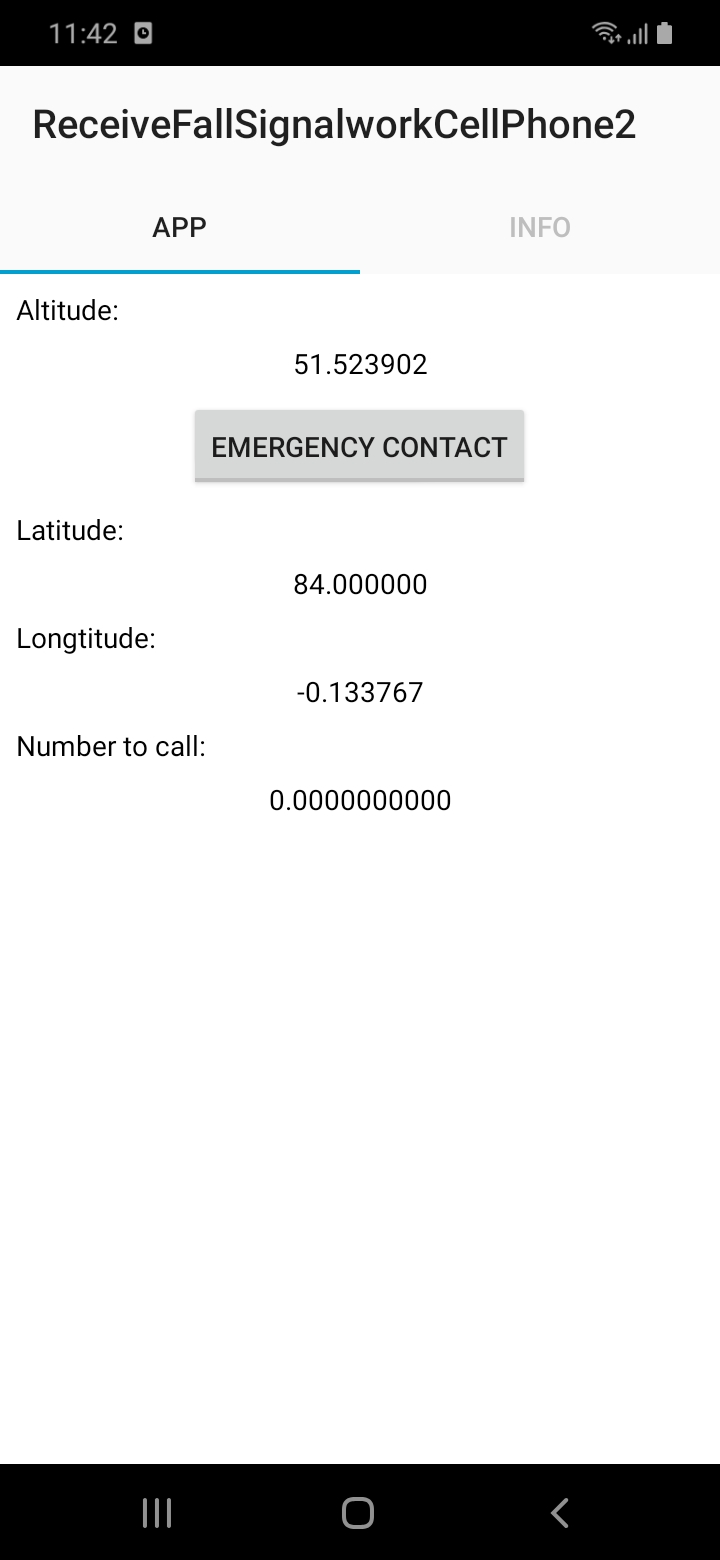
\includegraphics[width=\textwidth]{files/Interface.jpeg}
        \caption{}
    \end{subfigure}
    \begin{subfigure}[t]{0.4\textwidth}
        \centering
        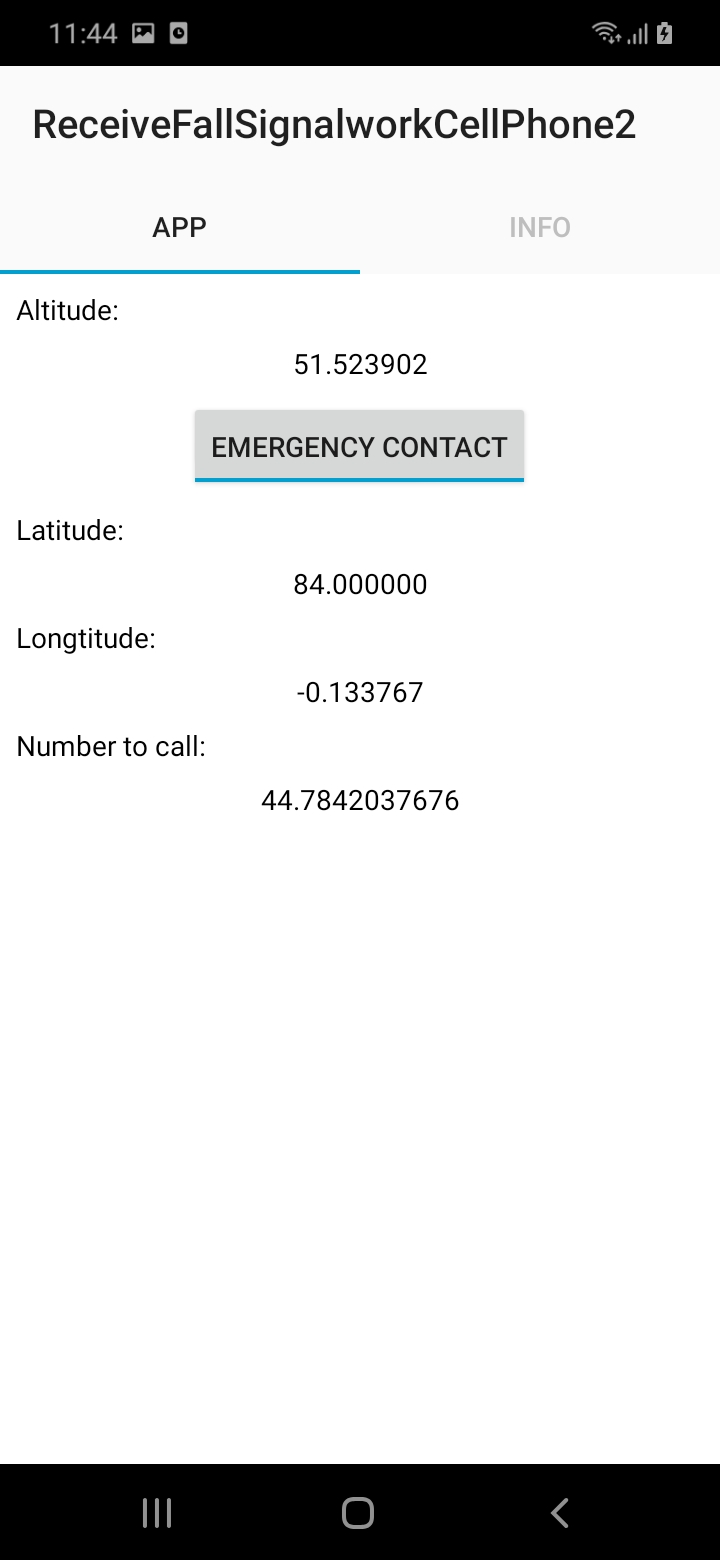
\includegraphics[width=\textwidth]{files/InterfaceTriggered.jpeg}
        \caption{}
    \end{subfigure}
    \caption{User interface of the \textit{receiver} phone. Note the information displayed is that of the \textit{sender}.}
\end{figure}
\paragraph{Future of the project}
    Many of our choices were designed based on the limitations of the software, and there is still a lot of room for improvement.
    Our main goals for the future are to implement this software into a wearable device such as a smartwatch or a bracelet.
    Additionally, the app should have the capability of directly calling the police or an ambulance in case of an emergency with the press of a button.
    The goal is to make this app the more convenient and easier to use for elderly people and their loved ones.  

\clearpage
\bibliography{bibliography}
\end{document}
